\chapter{Paramétrer le logiciel}
\section{Créer les lecteurs}
La liste des lecteurs peut être consultée depuis le menu \textit{Administration}  $\rightarrow$ \textit{Lecteurs}. 

\begin{figure}[H]
\centering
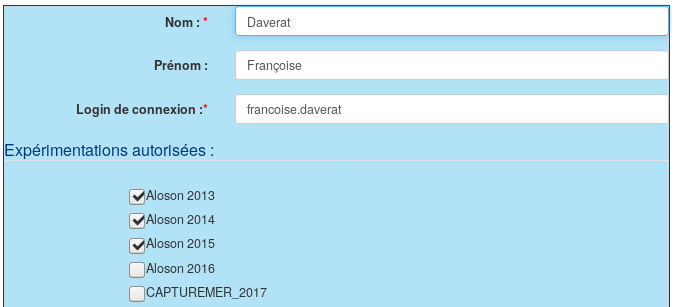
\includegraphics[width=0.7\linewidth]{images/lecteurs}
\caption{Détail d'un lecteur}
\end{figure}

Les informations à indiquer pour chaque lecteur sont les suivantes :
\begin{itemize}
\item son nom (obligatoire)
\item son prénom
\item son login de connexion (issu de la base de données interne ou de l'annuaire LDAP, le cas échéant)
\end{itemize}

Il suffit de cocher les expérimentations auxquelles il aura droit pour lui permettre de réaliser des lectures.


\section{Créer une expérimentation}
Les expérimentations sont les éléments de base de l'application. Elles sont utilisées pour gérer les droits attribués aux lecteurs.

Pour créer une expérimentation, choisissez \textit{Paramètres}  $\rightarrow$ \textit{Expérimentations}. Vous pouvez modifier une expérimentation existante ou en créer une nouvelle.

\begin{figure}[H]
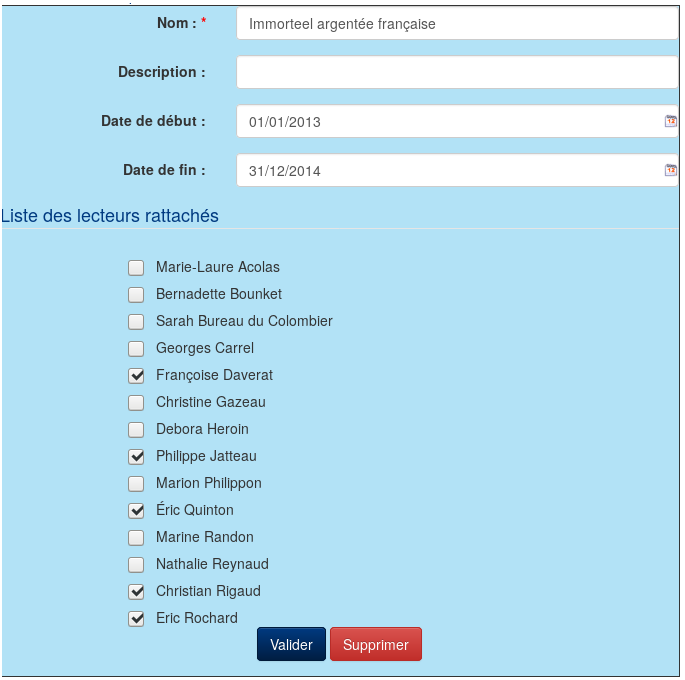
\includegraphics[width=\linewidth]{images/experimentation}
\caption{Écran de saisie/modification d'une expérimentation}
\end{figure}

La liste des lecteurs potentiels est affichée, il suffit de sélectionner ceux qui seront retenus pour lire les photos de l'expérimentation considérée.

À noter que seul le nom de l'expérimentation est obligatoire.

\section{Importer des poissons et des pièces calcifiées}

Pour éviter une saisie qui peut être fastidieuse, le logiciel permet d'importer un lot de poissons et leurs pièces calcifiées associées. L'importation automatique des photos n'est par contre pas possible.

Pour importer des poissons, choisissez \textit{Lectures} $\rightarrow$ \textit{Import}. 

\begin{figure}[H]
\centering
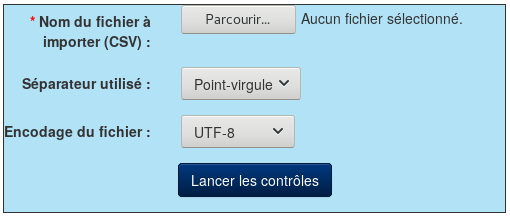
\includegraphics[width=0.7\linewidth]{images/import}
\caption{Écran de gestion des importations de poisson}
\end{figure}

L'importation est réalisée en deux étapes. Pendant la première, la conformité du fichier est vérifiée : si des anomalies sont détectées, elles sont affichées.

Si aucune anomalie n'est détectée, l'importation peut être déclenchée.

Voici la liste des colonnes qui peuvent être utilisées :

\begin{itemize}
\item \textbf{exp\_id} : code numérique de l'expérimentation (obligatoire)
\item  \textbf{espece\_id} : code de l'espèce (obligatoire)
\item     \textbf{tag} : N° de l'étiquette posée sur le poisson (le \textit{codeindividu} ou le \textit{tag} sont obligatoires)
\item     \textbf{codeindividu} : identifiant du poisson ou hptag
\item     \textbf{sexe\_id} : sexe du poisson (1 : mâle, 2 : femelle, 3 : juvénile, 4 : indifférencié)
 \item    \textbf{longueur} : longueur du poisson (mm)
\item     \textbf{poids} : poids du poisson (g)
 \item    \textbf{remarque} : remarques concernant le poisson
\item     \textbf{parasite} : parasites éventuels rencontrés
   \item  \textbf{age} : âge du poisson
  \item   \textbf{piecetype\_id} : code du type de pièce calcifiée à analyser Consultez la liste des types de pièces
   \item  \textbf{piececode} : si le type de pièce est indiqué, vous pouvez renseigner un code spécifique attaché à la pièce
  \item   \textbf{peche\_date} : date de la pêche, au format aaaa-mm-dd ou dd/mm/aaaa
   \item  \textbf{site} : site de la pêche
  \item   \textbf{zonesite} : zone précise de la pêche (précision concernant le site)
   \item  \textbf{campagne} : campagne de pêche
  \item   \textbf{peche\_engin} : engin utilisé, sous forme textuelle
   \item  \textbf{personne} : références du pêcheur
   \item  \textbf{operateur} : références de l'opérateur ayant traité le poisson
\end{itemize}

les dernières informations (site, zonesites, etc.) sont stockées sous forme de chaîne de caractères, il n'y a pas de tables qui leur sont dédiées.

\subsection{Modèle de fichier}

Un modèle de fichier utilisable pour l'importation peut être téléchargé. Le lien figure en bas de la page web.

\section{Gérer les tables de paramètres}
Deux tables de paramètres sont accessibles depuis l'application : la table des types de pièces calcifiées et la table des espèces. 

\subsection{Table des espèces}

La liste des espèces gérées par le logiciel est accessible depuis le menu \textit{Paramètres} $\rightarrow$ \textit{Espèces}. Il est possible de modifier ou rajouter un taxon (nom latin et nom français uniquement) :

\begin{figure}[H]
\centering
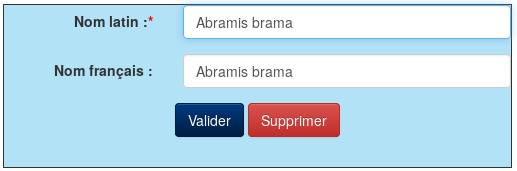
\includegraphics[width=0.5\linewidth]{images/espece}
\caption{Écran de modification d'un taxon}
\end{figure}

Le code affiché dans la liste est celui à utiliser pour les importations.

\subsection{Table des types de pièces calcifiées}

La liste des types de pièces peut être étendue depuis le menu \textit{Paramètres} $\rightarrow$ \textit{Pièces}. Seul le nom de la pièce est à indiquer.

\begin{figure}[H]
\centering
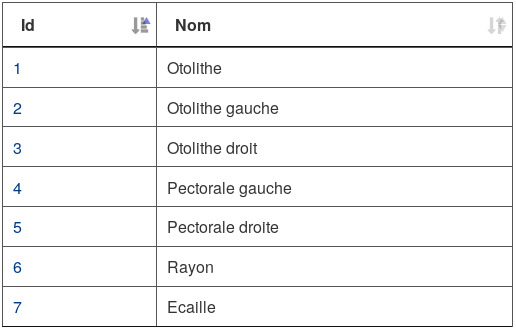
\includegraphics[width=0.5\linewidth]{images/piece}
\caption{Liste des types de pièces calcifiées}
\end{figure}

Le code affiché (colonne \textit{Id}) est celui à utiliser pour les importations.

